\documentclass[Royal,times,sageh]{sagej}

\usepackage{moreverb,url,natbib, multirow, tabularx}
\usepackage[colorlinks,bookmarksopen,bookmarksnumbered,citecolor=red,urlcolor=red]{hyperref}



% tightlist command for lists without linebreak
\providecommand{\tightlist}{%
  \setlength{\itemsep}{0pt}\setlength{\parskip}{0pt}}



\usepackage{booktabs}
\usepackage{longtable}
\usepackage{array}
\usepackage{multirow}
\usepackage{wrapfig}
\usepackage{float}
\usepackage{colortbl}
\usepackage{pdflscape}
\usepackage{tabu}
\usepackage{threeparttable}
\usepackage{threeparttablex}
\usepackage[normalem]{ulem}
\usepackage{makecell}
\usepackage{xcolor}


\begin{document}


\setcitestyle{aysep={,}}

\title{TTS2016R: A dataset to study population and employment patterns
from the 2016 Transportation Tomorrow Survey (TTS) in the Greater
Toronto and Hamilton Area, Canada}

\runninghead{}

\author{Anastasia Soukhov\affilnum{}, Antonio Páez\affilnum{}}

\affiliation{\affilnum{}{}}



\begin{abstract}
This paper describes and visualises the data contained within the
\{TTS2016R\} data package created in \texttt{R}, the statistical
computing and graphics language. In addition to a synthetic example,
\{TTS2016R\} contains home-to-work commute information for the Greater
Golden Horseshoe (GGH) area in Canada retrieved from the 2016
Transportation Tomorrow Survey (TTS). Included are all Traffic Analysis
Zones (TAZ), the number of people who are employed full-time per TAZ,
the number of jobs per TAZ, the count of origin destination (OD) pairs
and trips by mode per origin TAZ, calculated car travel time from TAZ OD
centroid pairs, and associated spatial boundaries to link TAZ to the
Canadian Census. To illustrate how this information can be analysed to
understand patterns in commuting, we estimate a distance-decay curve
(i.e., impedance function) for the region. The value in \{TTS2016R\} is
that it is a growing open data product built on \texttt{R}
infrastructure that allows for the immediate access of home-to-work
commuting data alongside complimentary objects from different sources.
The package will continue expanding with additions by the authors and
the community at-large by requests in the future. \{TTS2016R\} can be
freely explored and downloaded in the associated
\href{https://github.com/soukhova/TTS2016R}{Github repository} where the
documentation and code involved in data creation (including this
manuscript), manipulation, and all open data products are detailed.
\end{abstract}

\keywords{Jobs; population; work; commute; travel time; impedance;
Greater Toronto and Hamilton Area; Ontario, Canada; R}

\maketitle

\hypertarget{introduction}{%
\section{Introduction}\label{introduction}}

This manuscript presents the open data product
\href{https://github.com/soukhova/TTS2016R}{\{TTS2016R\}}. Open data
products are the result of turning source data (open or otherwise) into
accessible information that adds value to the original inputs
\citep[see][]{Arribas2021open}. The product presented in this paper is a
\texttt{R} data package which currently consists of a fusion of objects
from a variety of sources: home-to-work flows sourced from the 2016
Transportation Tomorrow Survey (TTS)
\citep{data_management_group_tts_2018}, estimated travel times
(calculated using \{r5r\} \citep{Pereira2021r5r}), and boundary files
from the TTS \citep{datamanagementgroupSurveyBoundaryFiles2018} and from
the Canadian Census \citep{statisticscanadaBoundaryFiles20162017}.

What is a \texttt{R} data package? A \texttt{R} data package contains
code, data, and documentation in a standardised collection format that
can be installed by \texttt{R} users through a centralized software
repository such as CRAN (the Comprehensive R Archive Network) and
GitHub. \{TTS2016R\} is freely available on GitHub for all to install
and freely use in the spirit of open and reproducible research.
Currently and in more detail, \{TTS2016R\} includes full-time home-based
work-to-job origin destinations (OD) counts and mode-specific trip
numbers retrieved from the 2016 TTS, traffic analysis zone (TAZ)
boundaries, and municipality, planning, and census metropolitan area
boundaries for the Greater Golden Horse area (GGH) located in southern
Ontario, Canada. In addition, the package includes TAZ
centroid-to-centroid travel times by car, transit, cycling, and walking
mode computed using package \{r5r\} \citep{Pereira2021r5r}.

The aim of this paper is to walk readers through the data sets,
illustrate a use case (i.e., the calculation of an impedance function
that can be used to calculate accessibility to employment), and invite
others to experiment in its uses and applications. Though data from the
TTS is freely available to the public through the
\href{https://dmg.utoronto.ca/idrs/index}{TTS Data Retrieval System},
the raw data can be technically demanding, cumbersome to work with, and
requires multiple software to process. By pre-processing the data,
packaging it with complimentary data, and providing explicit
documentation in a \texttt{R} environment, \{TTS2016R\} offers a slice
of the TTS data that can be immediately used by \texttt{R} users to
analysis patterns of commuting to work in the region. Anticipate this
package to grow in the future: it currently provides an open
infrastructure for additional TTS or complimentary data sets to be
amended by the authors and the open-source community in the future by
request.

\hypertarget{home-to-work-commute-data}{%
\section{Home-to-work commute data}\label{home-to-work-commute-data}}

Currently, \{TTS2016R\} includes counts of full-time employed population
by place of residence (origin), counts of full-time usual place of work
(destination), number of trips to work by mode, and the calculated
potential travel time of the trips in the GGH. The GGH (and hence the
TTS survey area) is displayed in Figure \ref{fig:TTS-16-survey-area}.

This data is aggregated and available at the level of TAZ: TAZ are a
spatial unit of analysis typically used to estimate the number of trips
produced and attracted to each zone \citep{meyer_urban_2001}. They are
thus defined by transportation planners for a region based on
intra-similarity and inter-dissimilarity between land-use and population
demographics. Within the GGH boundaries, 3,764 TAZ are specified and
each TAZ is uniquely identified using the GTA06 Zoning System: the
survey boundary is discussed in the 2016 TTS methodology and defined by
the TTS \citep{data_management_group_tts_2018}. The TAZ range between
\(\ge\) 0.019 km\textsuperscript{2} in spatial area to a maximum of 879
km\textsuperscript{2} (median: 1.3 km\textsuperscript{2} and 3rd
quantile: 2.8 km\textsuperscript{2}).

\begin{figure}[H]

{\centering 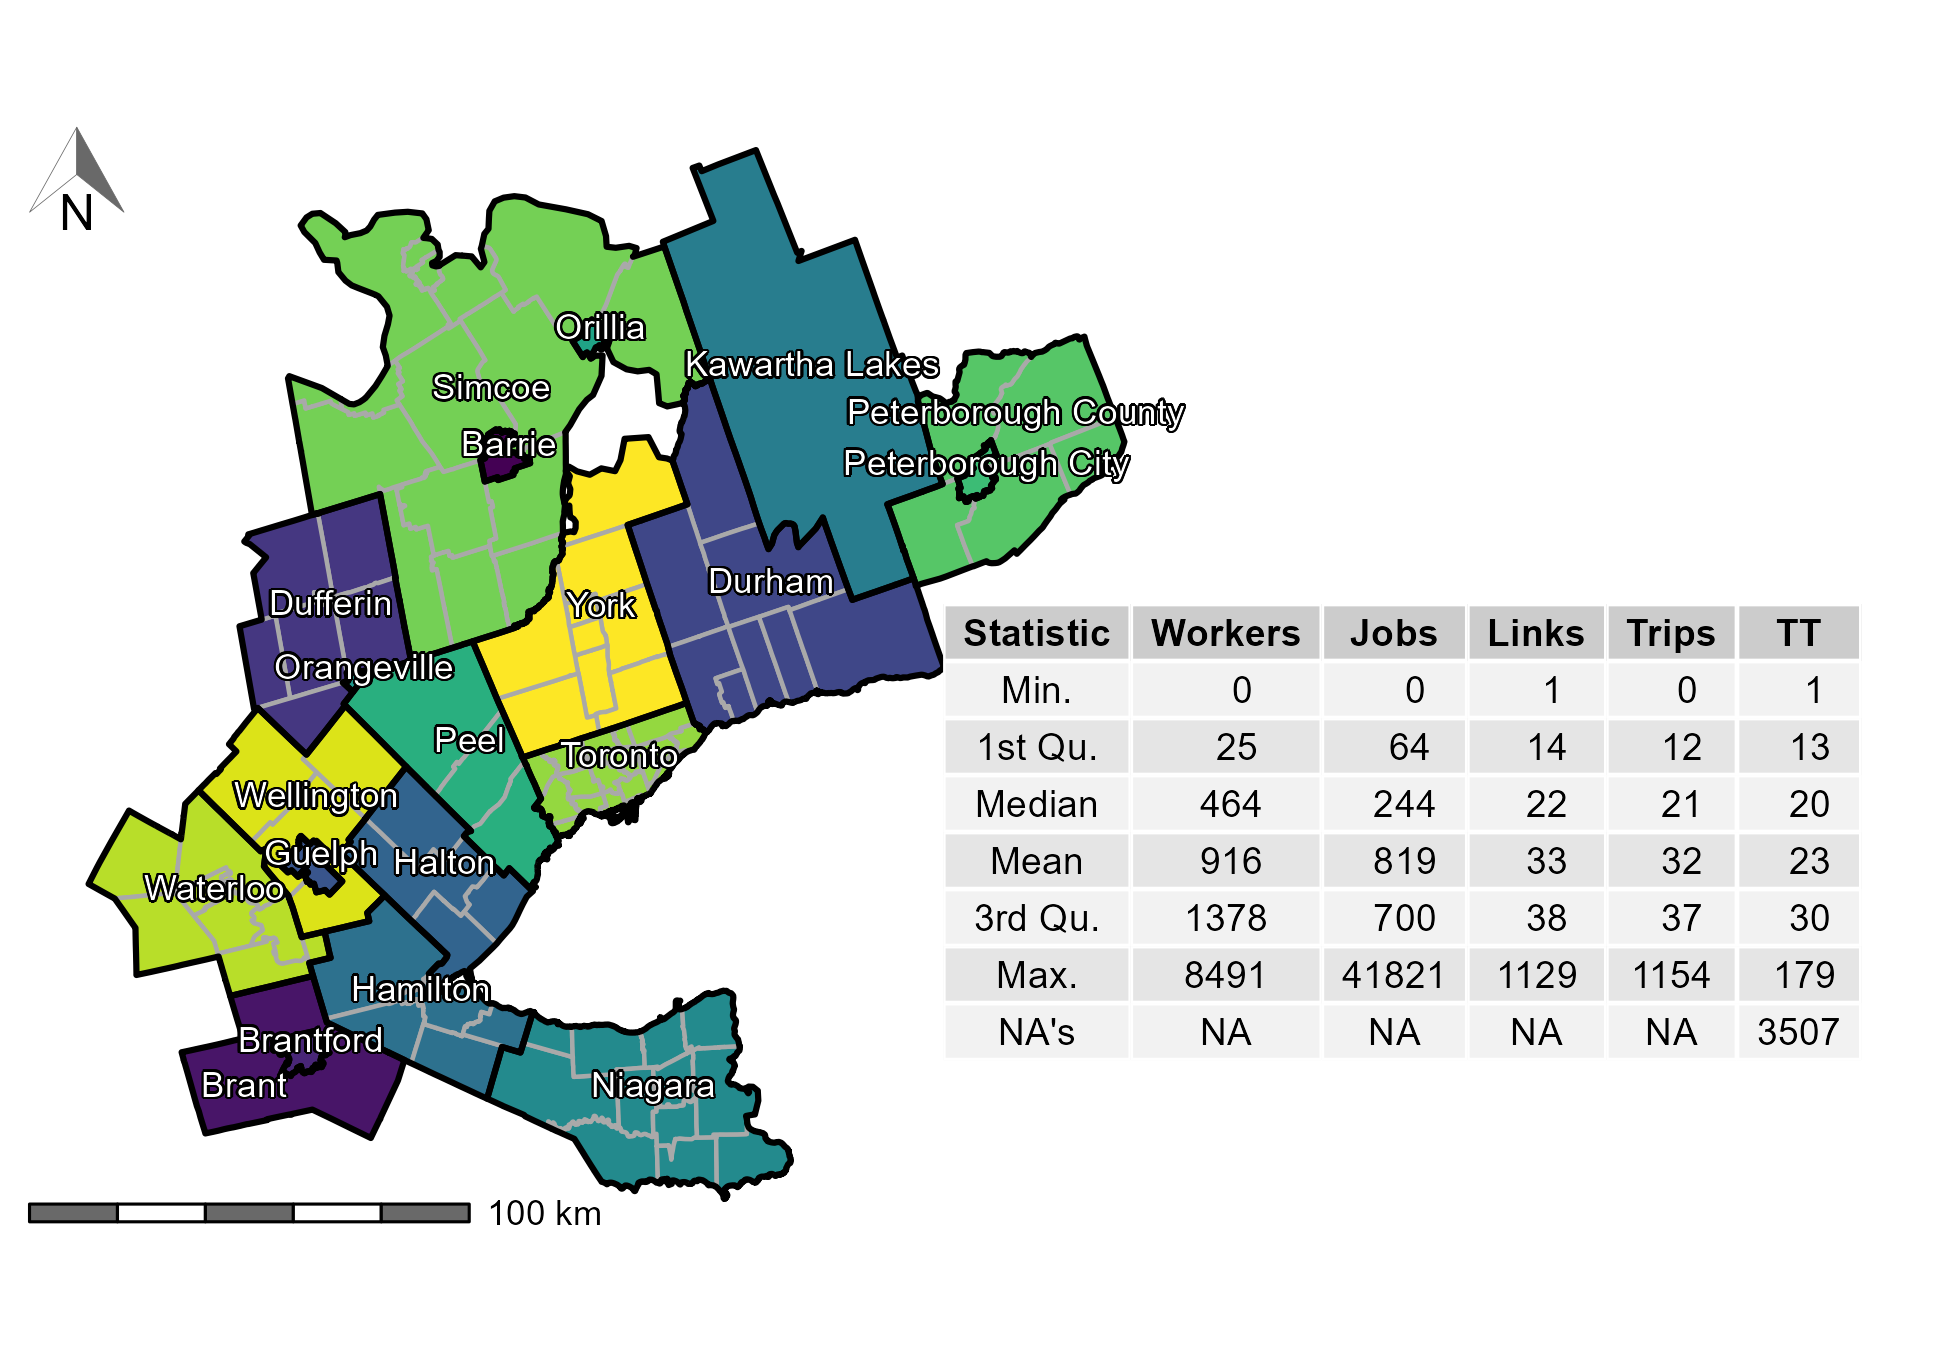
\includegraphics[width=1\linewidth]{images/TTS16-survey-area} 

}

\caption{\label{fig:TTS-16-survey-area}TTS 2016 study area within the GGH in Ontario, Canada along with associated descriptive statistic of workers and jobs per TAZ, OD links (count of workers potentially interacting with their place of employment) by origin TAZ, and calculated OD car travel time (TT) per origin TAZ. 3,507 trips were not assigned TT as they are longer than 180 mins. Spatial boundary files are retrieved from the TTS which define the survey area (Data Management Group, 2018a): the 20 regions in the GGH are represented by black lines and labelled, the dark gray lines are planning boundaries.}\label{fig:TTS-16-survey-area}
\end{figure}

\hypertarget{full-time-employed-people-and-associated-places-of-employment}{%
\subsection{Full-time employed people and associated places of
employment}\label{full-time-employed-people-and-associated-places-of-employment}}

In the GGH, there are 3,446,957 workers, 3,081,900 jobs, and 3,282,611
work-related trips (for the 2016 TTS survey day). The values are
organized within the origin destination (OD) table in the \{TTS2016R\}
package and are derived from the cross-tabulation by person and by trip
for the full-time employed population and associated places of
employment. The TTS is a proportionally representative survey, hence the
values included in \{TTS2016R\} are adjusted to reflect the GGH
population.

It is important to note that the total number of full-time workers and
jobs in the TTS 2016 region are not equal. Since the outer boundaries of
the TTS are permeable, workers who reside within the boundaries but have
workplaces that are outside of the boundaries are counted as workers
within an origin TAZ, while jobs in TAZ that are filled by workers who
reside outside the GGH boundaries are \emph{unknown} since they were not
surveyed. This mismatch results in the total number of workers being
1.12 times larger than the number of jobs (i.e., 3,446,957 workers to
3,081,900 jobs). As such, the OD table contained in \{TTS2016R\} offers
a perspective on all workers in the GGH and their home-based trips to
places of GGH employment.

The count of links and trips made by the full-time working population
and associated full-time place of employment per unique OD pair are
quite variable. TAZ contain between 0 to 8,491 workers (median: 464, 3rd
quantile: 1,378), 0 to 41,821 jobs (median: 244, 3rd quantile: 700), and
generate between 0 to 241 trips (median: 15, 3rd quantile: 42).

\begin{figure}
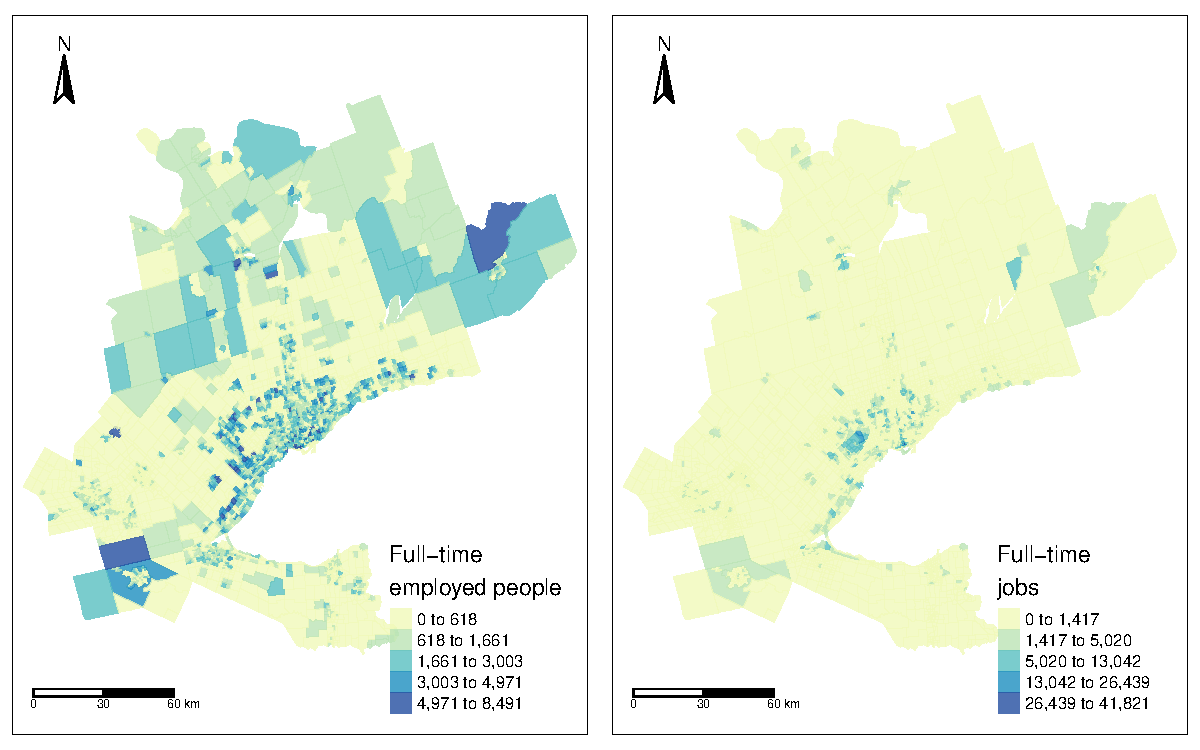
\includegraphics[width=1\linewidth]{Manuscript-Data-Package_files/figure-latex/tts-workers-jobs-plot-1} \caption{\label{fig:tts-workers-jobs-plot}Number of workers (left) and jobs (right) in each TAZ retrieved from the 2016 TTS (Data Management Group, 2018b). Spatial boundary files are retrieved from the TAZ defined by the TTS (Data Management Group, 2018a).}\label{fig:tts-workers-jobs-plot}
\end{figure}

Figure \ref{fig:tts-workers-jobs-plot} presents the number of employed
people and associated jobs per TAZ. It can be observed that the spatial
distribution of jobs and workers is unequal, which is indicative of a
jobs -housing imbalance that can impact accessibility in a region
\citep{Levine1998rethinking}. It can also be seen that there is a higher
number of TAZ with no workers than zones with no jobs (i.e., 791 TAZ
with no workers : 396 TAZ with no jobs) and the mean of workers per TAZ
is higher than the mean of jobs. The number TAZ with an extreme number
of jobs at the highest and lowest percentiles is significantly higher
than the number of workers.

\hypertarget{calculated-travel-time}{%
\subsection{Calculated travel time}\label{calculated-travel-time}}

Also included in \{TTS2016R\} are the estimated travel times between OD
as summarized in descriptive statistics table in Figure
\ref{fig:plot-tt-ttpertrip}; travel times are calculated using the
package \{r5r\}. \{r5r\} interfaces with the java-based R5 routing
engine developed separately by Conveyal
\citep{conveyalConveyalR5Routing2022}. The inputs to \{r5r\} for this
data package were the desired mode, a maximum travel time threshold of
180 minutes, the geo-coded origin destination pairs based on the
centroids of the TAZ, and the static Open Street Map road network of
Ontario (retrieved using Geofabrick
\citep{geofabrikOntarioOpenStreetMapGeofabrik2022}). A travel time
threshold of 180 minutes was selected since it captures almost all
potential OD interactions.

Additionally, the car mode was included since it is a critically
important commute mode in the GGH. 2,598,379 of the trips are made using
a car mode out of the total 3,282,611 work-related trips according to
the TTS 2016 data (i.e., 79\% of trips are taken by car).

These travel times are useful addition to \{TTS2016R\} since they are
not included in the TTS Data Retrieval System but they are vitally
important to estimate the cost of travel and associated impedance
functions, among other possible applications. If the readership is
interested in additional information regarding the travel time
computation, please see the calculation notebook in the documentation of
\{TTS2016R\} and details about \{r5r\} at the
\href{https://ipeagit.github.io/r5r/index.html}{r5r package website}.

\begin{figure}
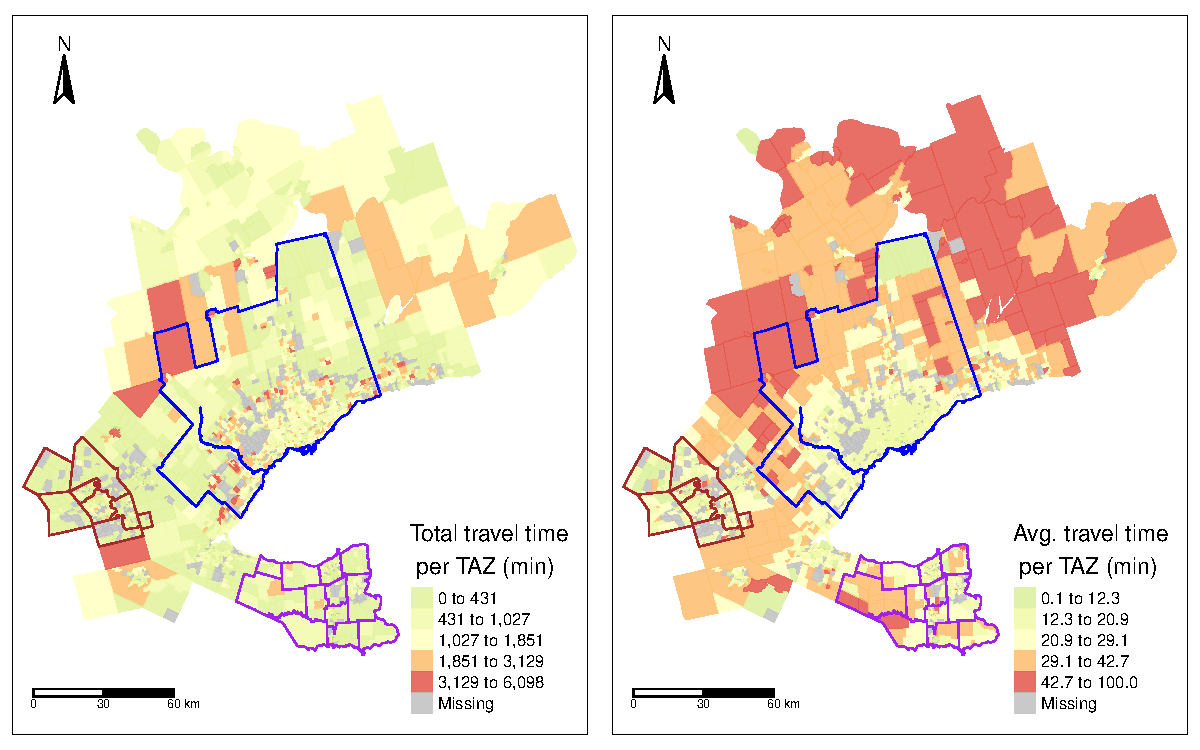
\includegraphics[width=1\linewidth]{Manuscript-Data-Package_files/figure-latex/plot-tt-ttpertrip-1} \caption{\label{fig:plot-tt-ttpertrip}Calculated total worker travel time (left) and average worker travel time (right) for each TAZ in the 2016 TTS. Planning boundaries of Niagara and Waterloo (Data Management Group, 2018a), and the Toronto census metropolitan area (Statistics Canada, 2017) are drawn with purple, brown and blue borders, respectively. }\label{fig:plot-tt-ttpertrip}
\end{figure}
\newpage

As can be observed in Figure \ref{fig:plot-tt-ttpertrip}, the total
travel time resembles the spatial trend distribution in the number of
employed people in the previous plot (Figure
\ref{fig:tts-workers-jobs-plot}) and the spatial distribution of the
average travel time is distinct from other plots presented so far. For
instance, we can see that in areas around the south-eastern border such
as Niagara and Waterloo (purple and brown borders), the average travel
times are moderately low. Additionally, travel times (by car) within the
core of the Toronto census metropolitan area (CMA) (blue) is also
moderately since traffic congestion is not reflected in the travel time
estimations. Further from these areas, travel times are higher.

\hypertarget{calibrating-an-impedance-function}{%
\subsection{Calibrating an impedance
function}\label{calibrating-an-impedance-function}}

Impedance functions are useful to understand mobility behaviour and are
used to estimate gravity models of spatial interaction
\citep{wilson1971, haynes_gravity_1985} and applied in accessibility
analysis
\citep{hansen_how_1959, talen_assessing_1998, paez_jobs_2013, barboza_balancing_2021}.
An impedance function \(f(\cdot)\) depends on the cost of travel
\(c_{ij}\) between locations \(i\) and \(j\) (all which is supplied in
the travel time and origin-destination table within \{TTS2016R\}).

A useful technique to calibrate an impedance function is to use the trip
length distribution (TLD) as measured from origin-destination data
\citep{horbachov_theoretical_2018, batista_estimation_2019}. The TLD is
the representation of the likelihood that a proportion of trips are
taken at a specific travel cost. In our data set, where we assume cost
is travel time, the impedance function maps low travel times to higher
proportions of trips, and high travel times are mapped to low proportion
of trips.

Using the data contained in \{TTS2016R\}, we fit the empirical TLD to a
density distribution using maximum likelihood techniques and the
Nelder-Mead method for direct optimization available within the
\texttt{R} package \{fitdistrplus\} \citep{fitdistrplus_2015}. Based on
goodness-of-fit criteria and diagnostics seen in Figure
\ref{fig:TLD-Gamma-plot}, the gamma distribution is selected. The
`shape' parameter is \(\alpha\) = 2.019, the estimated `rate' is
\(\beta\) = 0.094 , and \(\Gamma(\alpha)\) is defined in Equation
(\ref{gamma-dist}).

\begin{figure}

{\centering 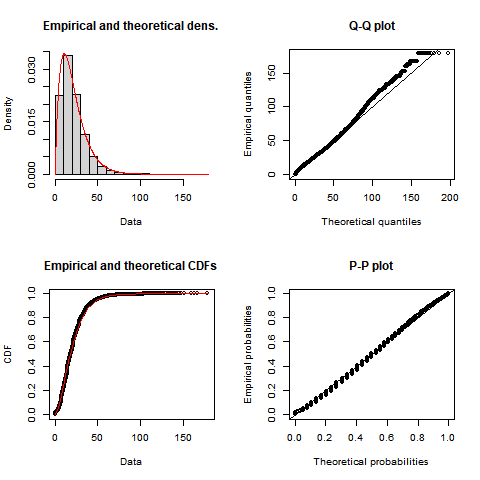
\includegraphics[width=0.75\linewidth]{images/impedance_function} 

}

\caption{\label{fig:TLD-Gamma-plot}Empirical TTS 2016 home-based car TLD (black) and calibrated gamma distribution impedance function (red) with associated Q-Q and P-P plots}\label{fig:TLD-Gamma-plot}
\end{figure}

\begin{equation}
\label{gamma-dist}
\begin{array}{l}\ 
f(x, \alpha, \beta) = \frac {x^{\alpha-1}e^{-\frac{x}{\beta}}}{ \beta^{\alpha}\Gamma(\alpha)} \quad \text{for } 0 \leq x \leq \infty\\
\Gamma(\alpha) =  \int_{0}^{\infty} x^{\alpha-1}e^{-x} \,dx\\
\end{array}
\end{equation}\textbackslash end\{equation\}

\newpage

\hypertarget{concluding-remarks}{%
\section{Concluding remarks}\label{concluding-remarks}}

\{TTS2016R\}, the open data package introduced in this paper fuses
multiple sources of data. It includes an OD cross-tabulation by person
and by trip mode table for home-to-work commute data from the 2016 TTS
alongside complimentary boundaries and estimated travel times. The value
of this data package is in its transparency, easy of access, and its
open infrastructure for the addition of complimentary data sets in the
future. Using \texttt{R} users can immediately and easily explore GGH
commute flow trends as well as suggestion further amendments to the
package by request. One possible use of this data, as showcased in this
paper, is the calibration of impedance functions which in turn can be
used for accessibility analysis.

In the spirit of novel and original research, we hope readers value the
efforts made to detail the data in order to improve transparency in our
work and encourage others to replicate and, hopefully, inspire research
of their own. We see this product as providing open infrastructure for
additional TTS or complimentary data sets to be amended by the authors
or wider open-source community in the future.

\bibliographystyle{sageh}
\bibliography{bibfile}


\end{document}
